\chapter{Preliminary Analysis} \label{App:preanalysis}
 - Pollutant correlation
 - extracting at monitoring stations
 - Pollutant metero correlation
 - AOD correlation
 - subregions/clusters?

\section{Pollutant Correlations and Relationships} \label{App:Corrs}
 
One of the first considerations for this project was the choice of air pollutant, as discussed in Sections \ref{Section:Motivation} and \ref{Section:Air Poll}, PM$_{2.5}$ was chosen for a number of different reasons, but it was important to consider other pollutants and how they interact with PM$_{2.5}$. Using the ground monitored data monthly means of PM$_{2.5}$, NO$_{2}$, SO$_{2}$, and O$_{3}$ for 2005-2020 we can see the relationships and correlations between them in Figure \ref{fig:pollcorr}. We can see that PM$_{2.5}$ is moderately positively correlated with NO$_{2}$ and SO$_{2}$, which can be explained by the overlap in sources of these pollutants, e.g. traffic-related pollution and industry, whereas O$_{3}$ has a inverse correlation to the other pollutants due having different sources and as ozone is a product of atmospheric chemical reactions involving other pollutants and UV, see Table \ref{table:2}.

\begin{figure}[h]
    \centering
    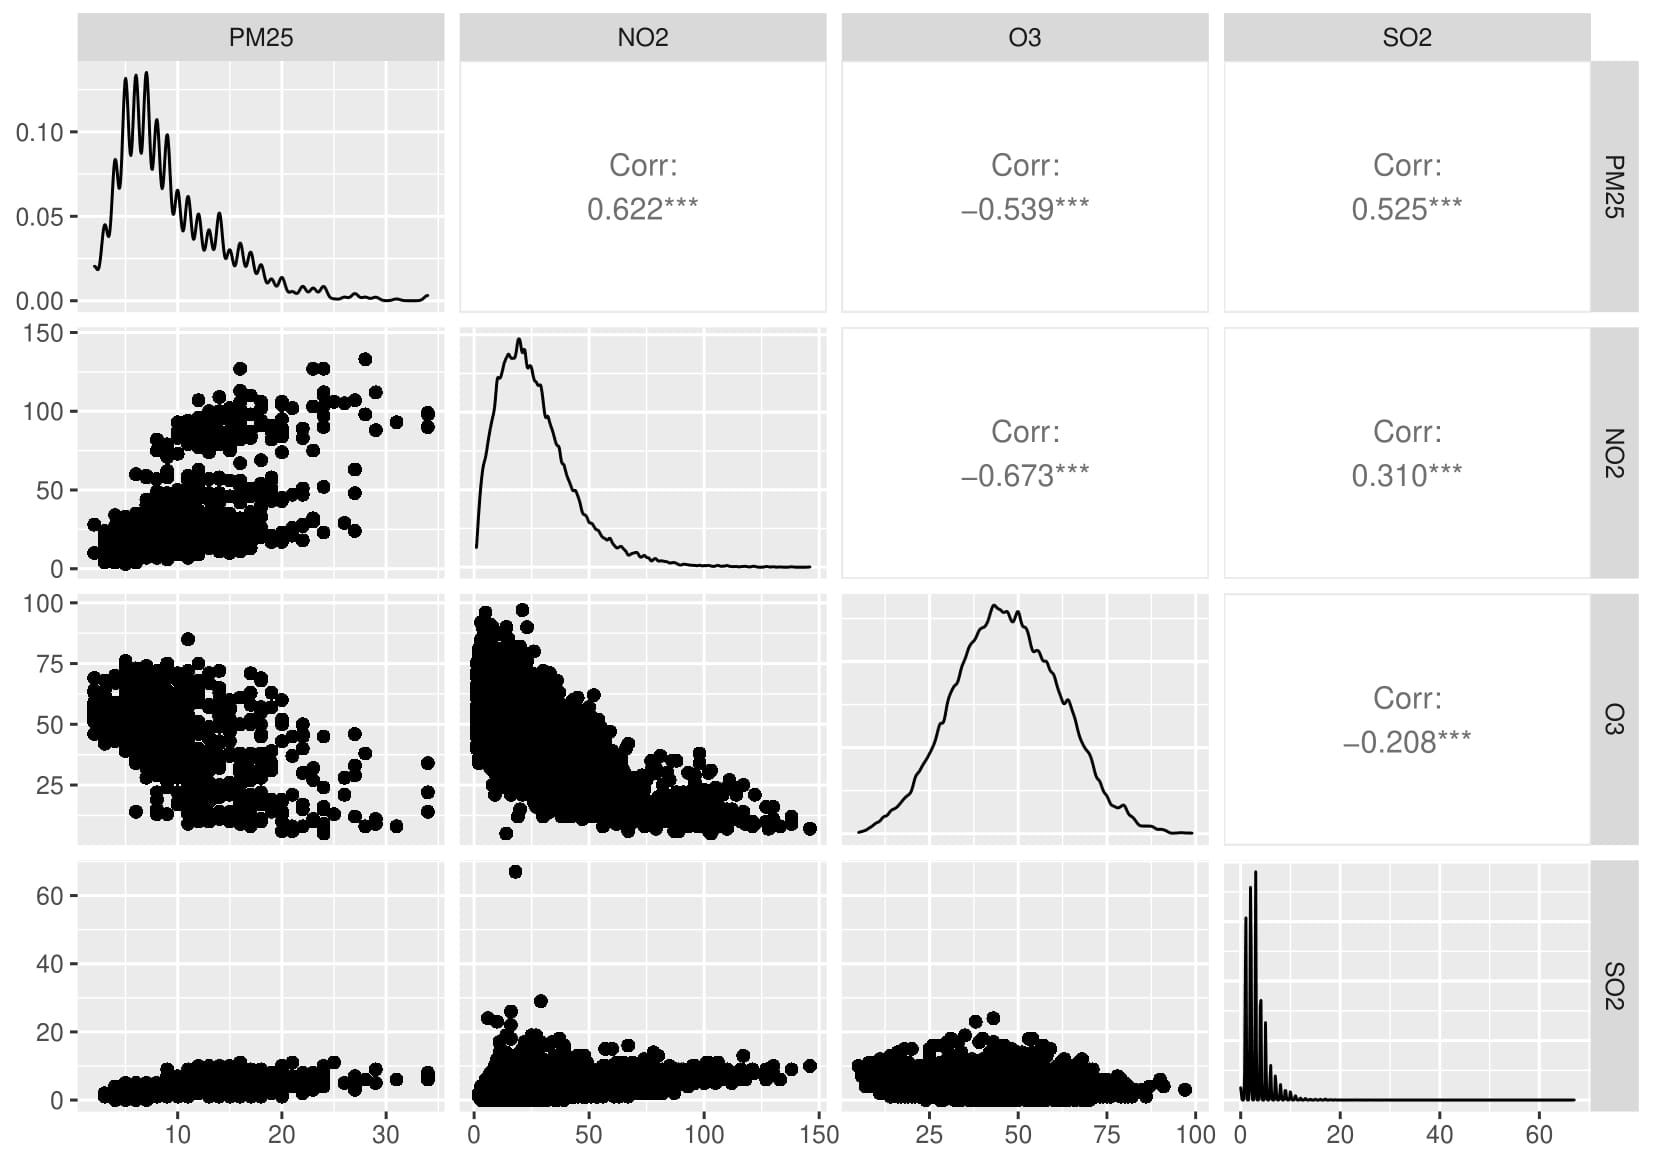
\includegraphics[width=1\textwidth]{Images/PollCorr-1.jpg}
    \caption{Relationships between ground monitored PM$_{2.5}$, NO$_{2}$, SO$_{2}$, and O$_{3}$}
    \label{fig:pollcorr}
\end{figure}

%hist of pm2.5 for different site types or regions
Another important feature of ground monitored pollution data, is the relation to site and environment type. The AURN monitoring stations are assigned one of 5 site types: rural background, suburban background, urban background, urban industrial, and urban traffic. We can see the distribution of PM$_{2.5}$ monthly mean levels for the UK by site type in Figure \ref{fig:pm25sites}. results...

\begin{figure}[h]
    \centering
    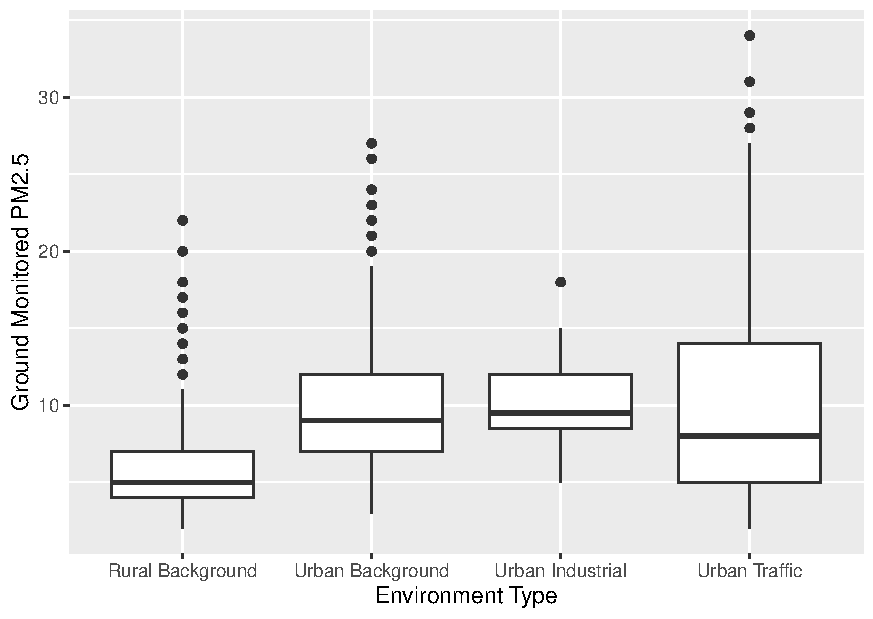
\includegraphics[width=1\textwidth]{Images/PM2.5 Boxplot.pdf}
    \caption{Ground Monitored PM$_{2.5}$ by site type}
    \label{fig:pm25sites}
\end{figure}

Another consideration is the use of meteorological variables as covariates within the exposure model, as seen in Section \ref{Section:Met Data} temperature, precipitation and humidity were chosen. These variables have been chosen for their correlation to pollutant concentrations and to represent the seasonality of air quality in the UK \citep{Hodgson2021SeasonalUK}. From the HadUK-Grid data, monthly mean meteorological data was extracted at each pollutant monitoring station for each month 2005-2020, correlation results can be seen in Figure \ref{fig:metcorr}. The resulting $R^2$ correlation values for PM$_{2.5}$ and the meterological variables is rather interesting, we see ..... However other studies have seen a much stronger linear correlation, such as humidity and temperature in \cite{Berrocal2020AConcentration}, which may be explained by the use of aggregated monthly means values of all variables here, so does not reflect extreme weather and pollution events, such as those seen in \cite{Kalisa2018TemperatureUK}, or there are more complicated relationships at play which need to be considered to use meteorology as a covariate to air pollution.

\begin{figure}[h]
    \centering
    \includegraphics[width=1\textwidth]{...}
    \caption{Relationships between ground monitored PM$_{2.5}$ and meteorological variables}
    \label{fig:metcorr}
\end{figure}

\section{Preliminary Time Series} \label{App:Time Series}
Time series analysis of the observed ground monitoring data for PM$_{2.5}$, shows a number of key preliminary findings of current and trending PM$_{2.5}$ concentrations across the UK. Figure \ref{fig:timesites} shows the raw observed time series plots for 12 PM$_{2.5}$ Monitoring Sites, which show very little ground monitored data prior to 2010 and some other smaller gaps in measurements at some sites.

\begin{figure}
    \begin{subfigure}{.5\textwidth}
        \centering
        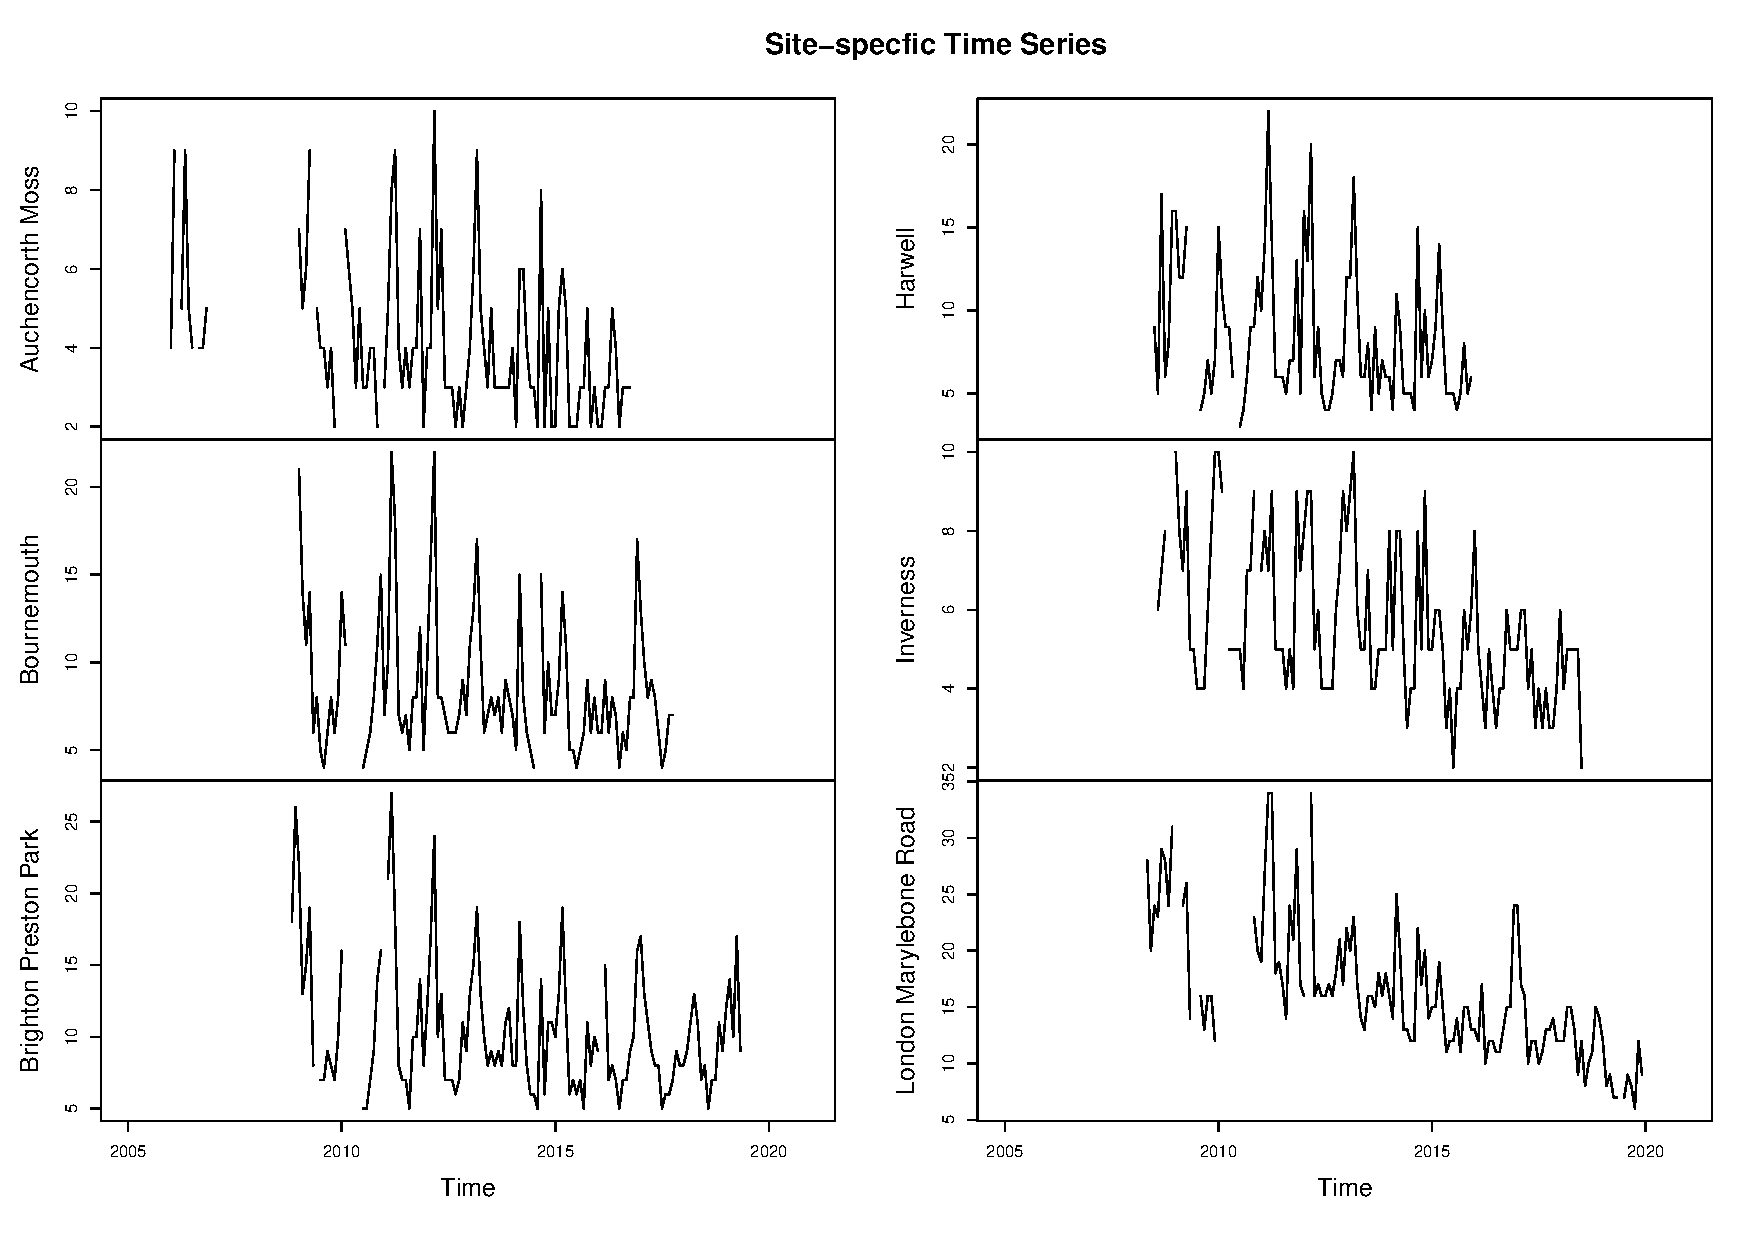
\includegraphics[width=\linewidth]{Images/Site ts 1.pdf}
    \end{subfigure}%
    \begin{subfigure}{.5\textwidth}
        \centering
        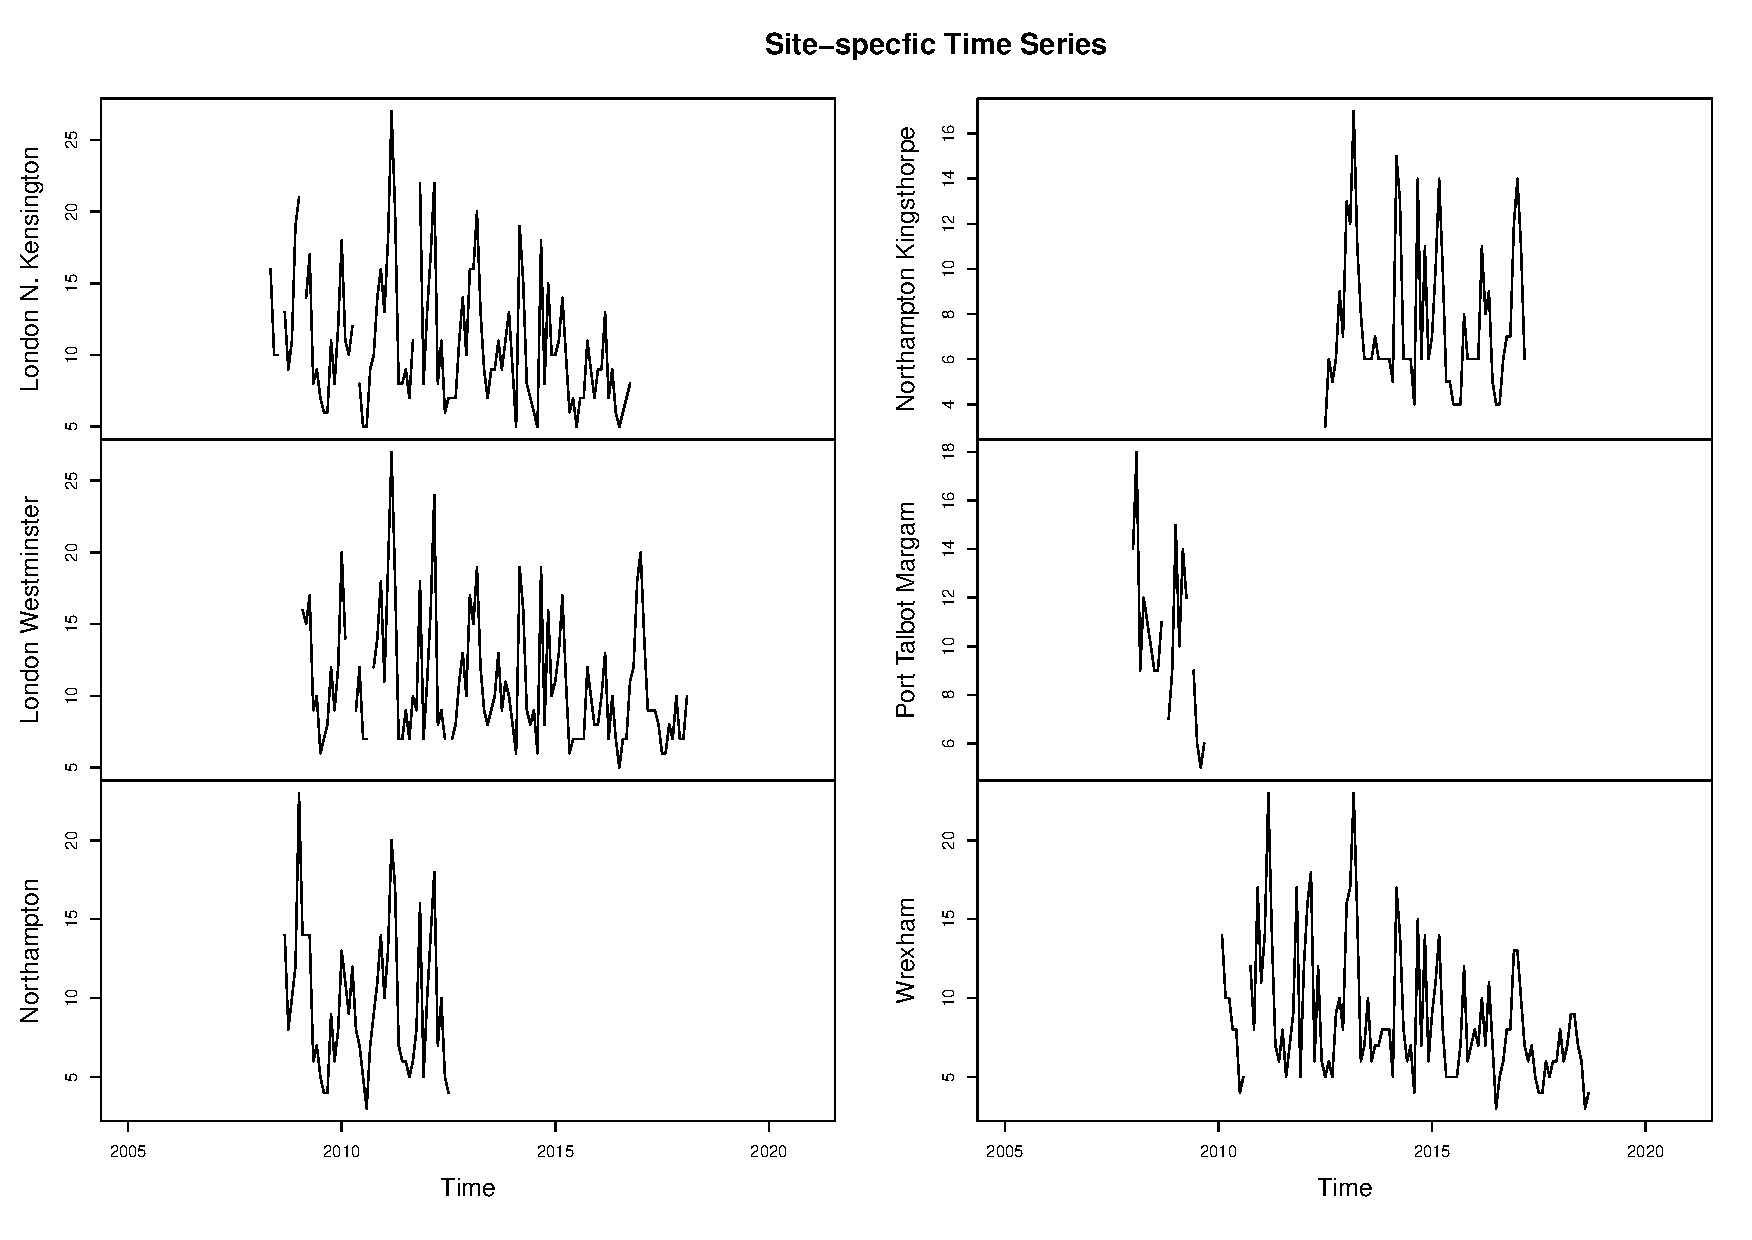
\includegraphics[width=\linewidth]{Images/Site ts 2.pdf}
    \end{subfigure}
\caption{Observed Time Series for 12 PM$_{2.5}$ Monitoring Sites}
\label{fig:timesites}
\end{figure}

Due to the nature of the air pollution situation and current literature, it is known that PM$_{2.5}$ concentrations do show heavy seasonality, as well as some significant changes year-to-year, as the pollution situation changes. Following from this, it is interesting to identify such seasonal and overall trends. Using the na.interp function from the forecast package in R, the missing time series data can be imputed through time-series interpolation that accounts for the overall seasonality of the data, see GitHub Repository \ref{GitHub}. Then using the decompose function, these interpolated time series can be decomposed into the overall trend, the seasonal trend, and the observed errors, Figure \ref{fig:decompts} shows the decomposed additive time series for 4 monitoring stations: Brighton Preston Park (Figure \ref{fig:BPPts}), London Marylebone Road (Figure \ref{fig:LMRts}), London Westminster (Figure \ref{fig:LWts}), and Wrexham (Figure \ref{fig:Wts}).

\begin{figure}
    \begin{subfigure}{.5\textwidth}
        \centering
        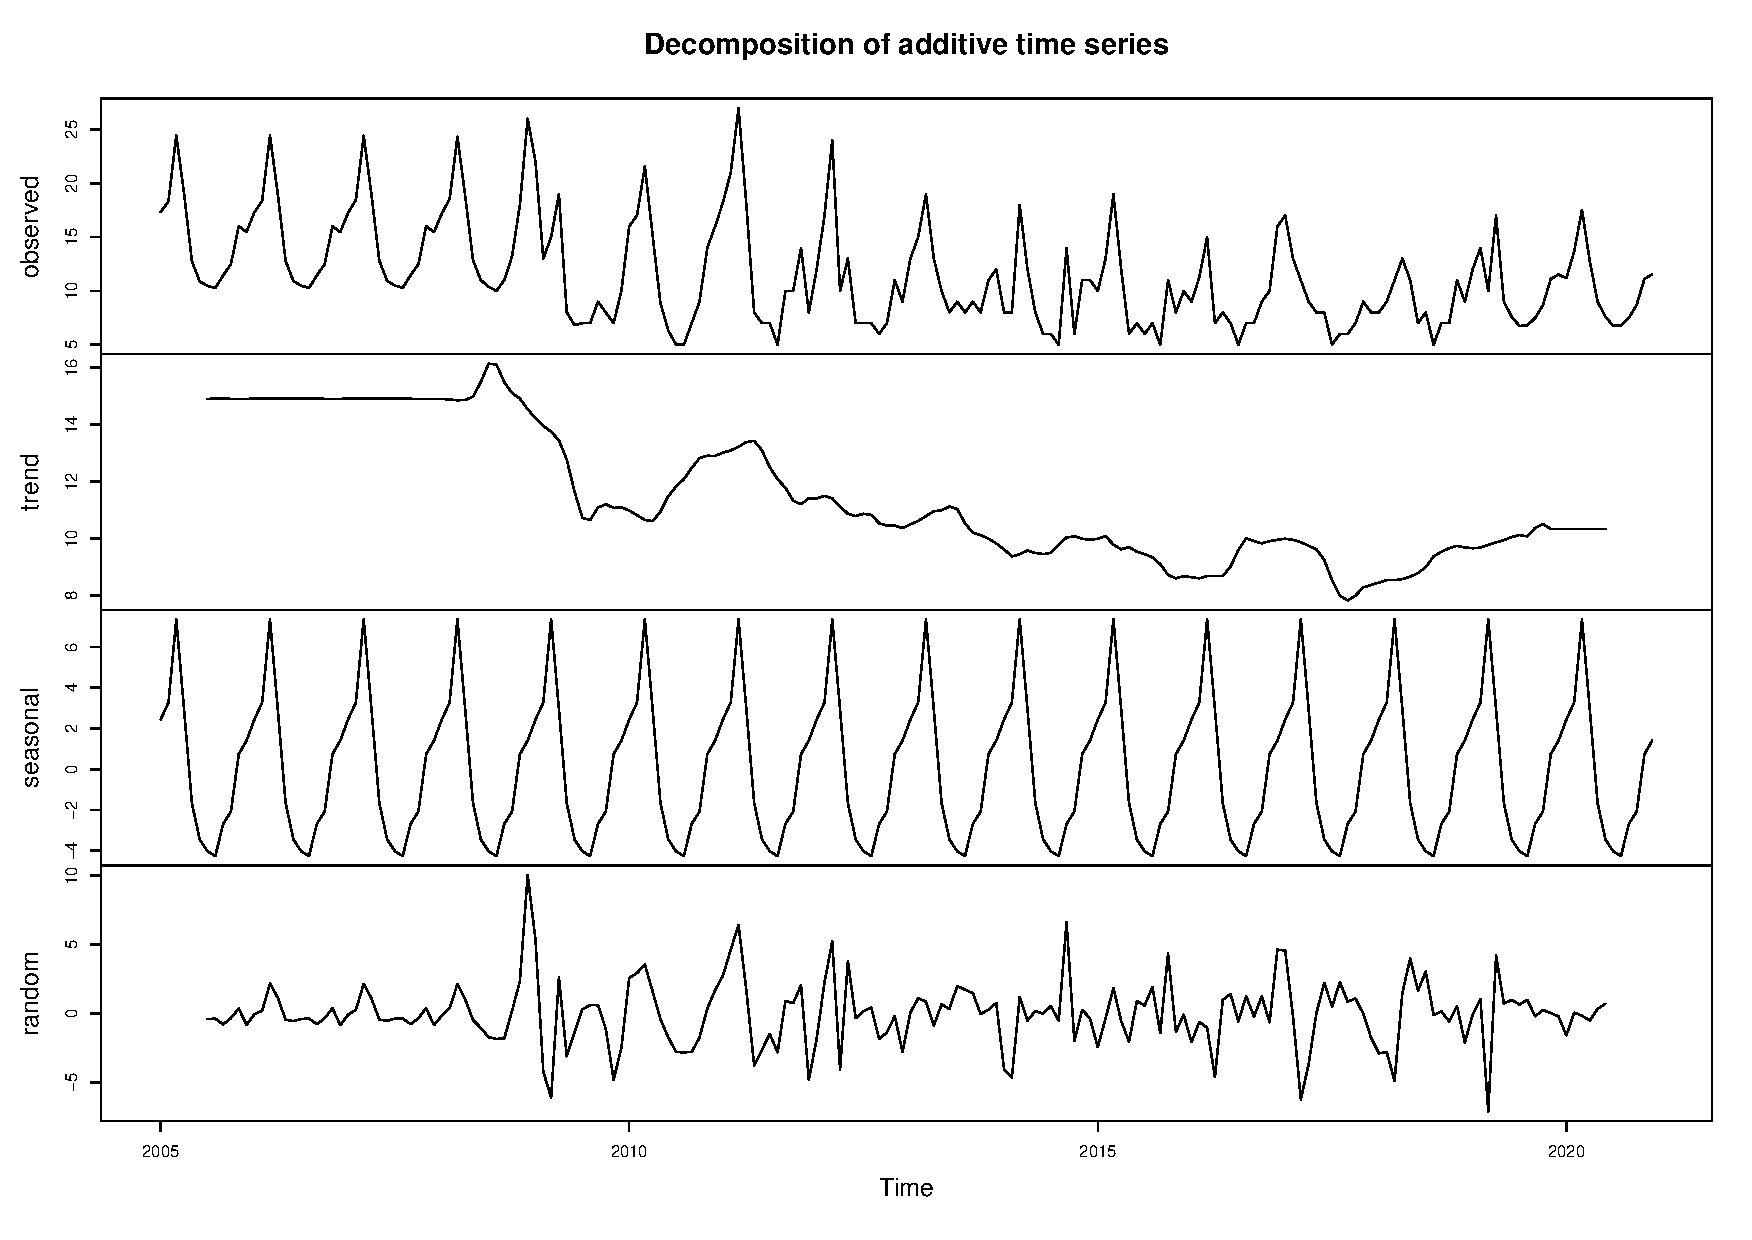
\includegraphics[width=\linewidth]{Images/Brighton Preston Park ts.pdf}
        \caption{Decomposed Additive Time Series for Brighton Preston Park}
        \label{fig:BPPts}
    \end{subfigure}%
    \begin{subfigure}{.5\textwidth}
        \centering
        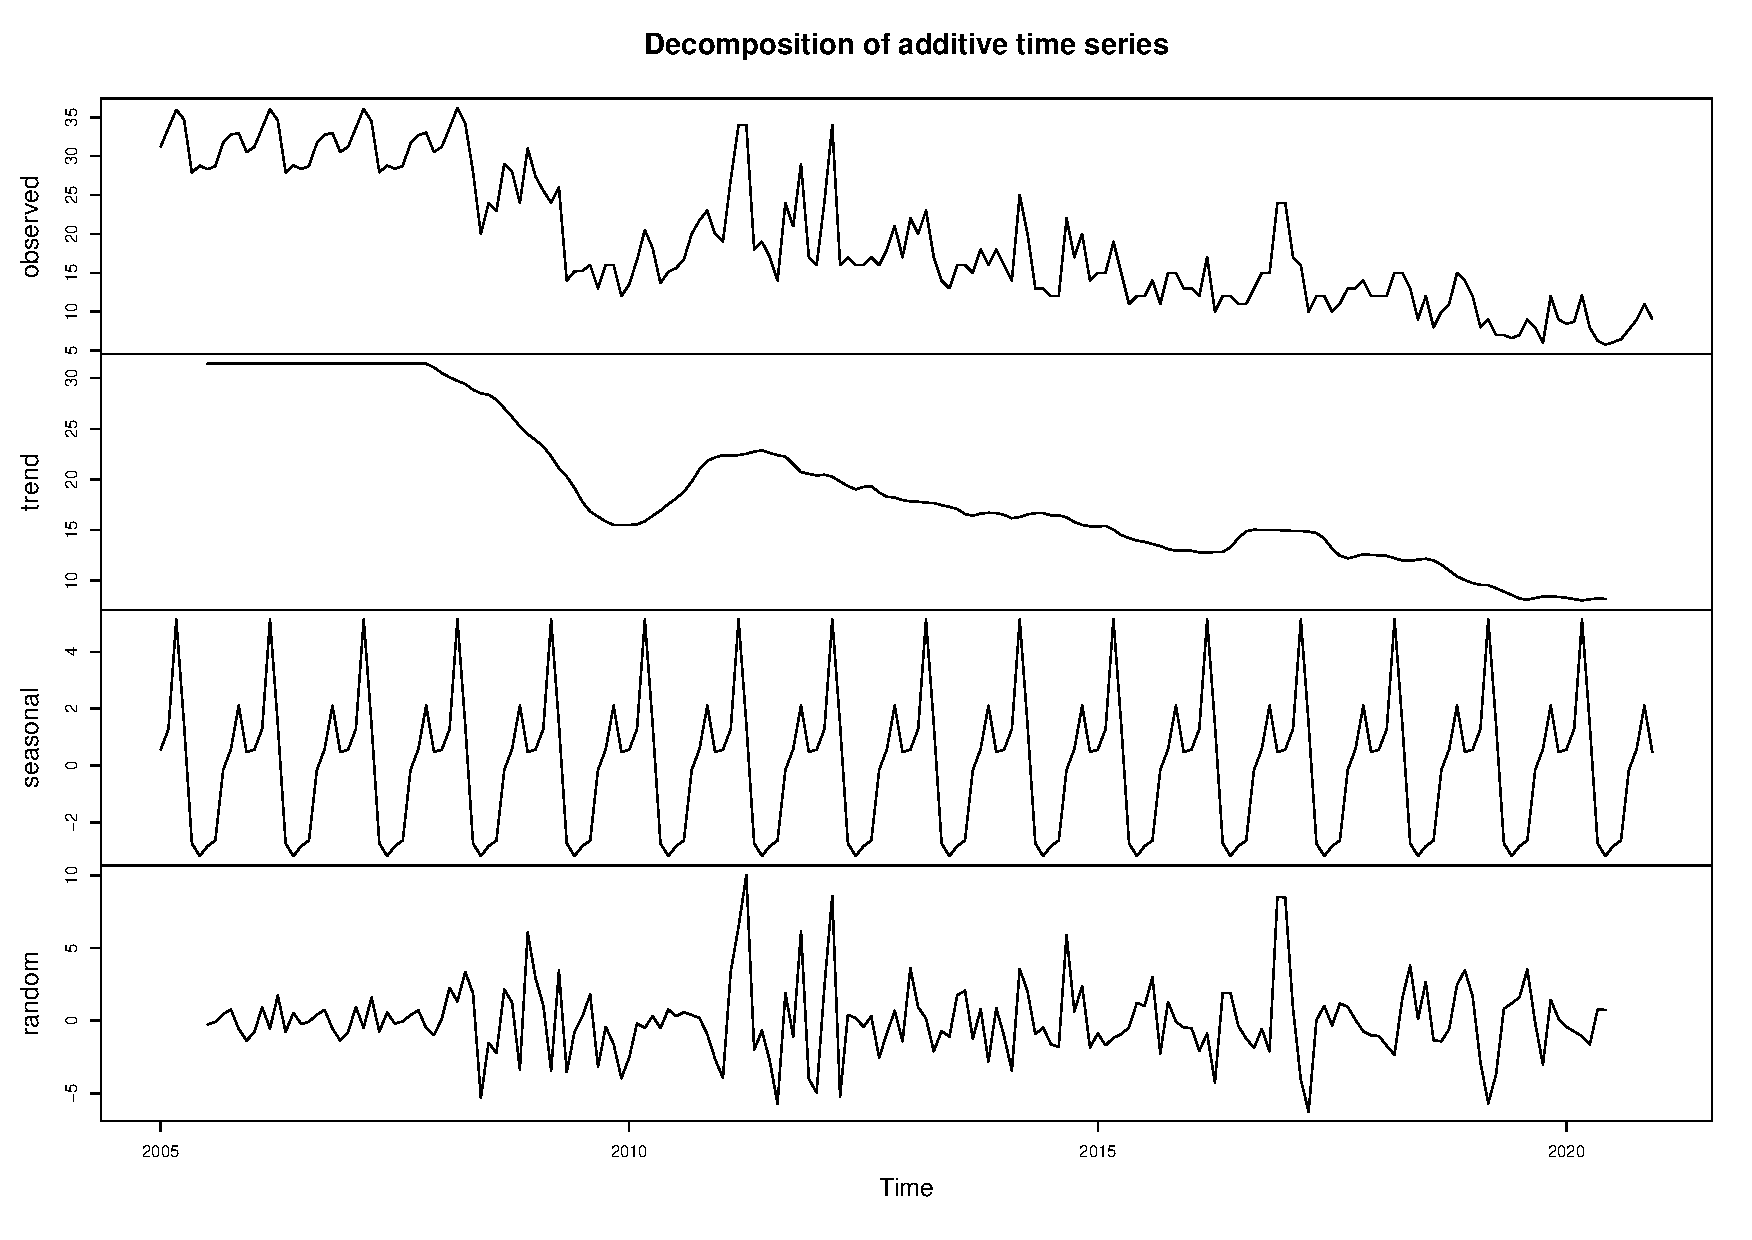
\includegraphics[width=\linewidth]{Images/London Marylebone Road ts.pdf}
        \caption{Decomposed Additive Time Series for London Marylebone Road}
        \label{fig:LMRts}
    \end{subfigure}
    \begin{subfigure}{.5\textwidth}
        \centering
        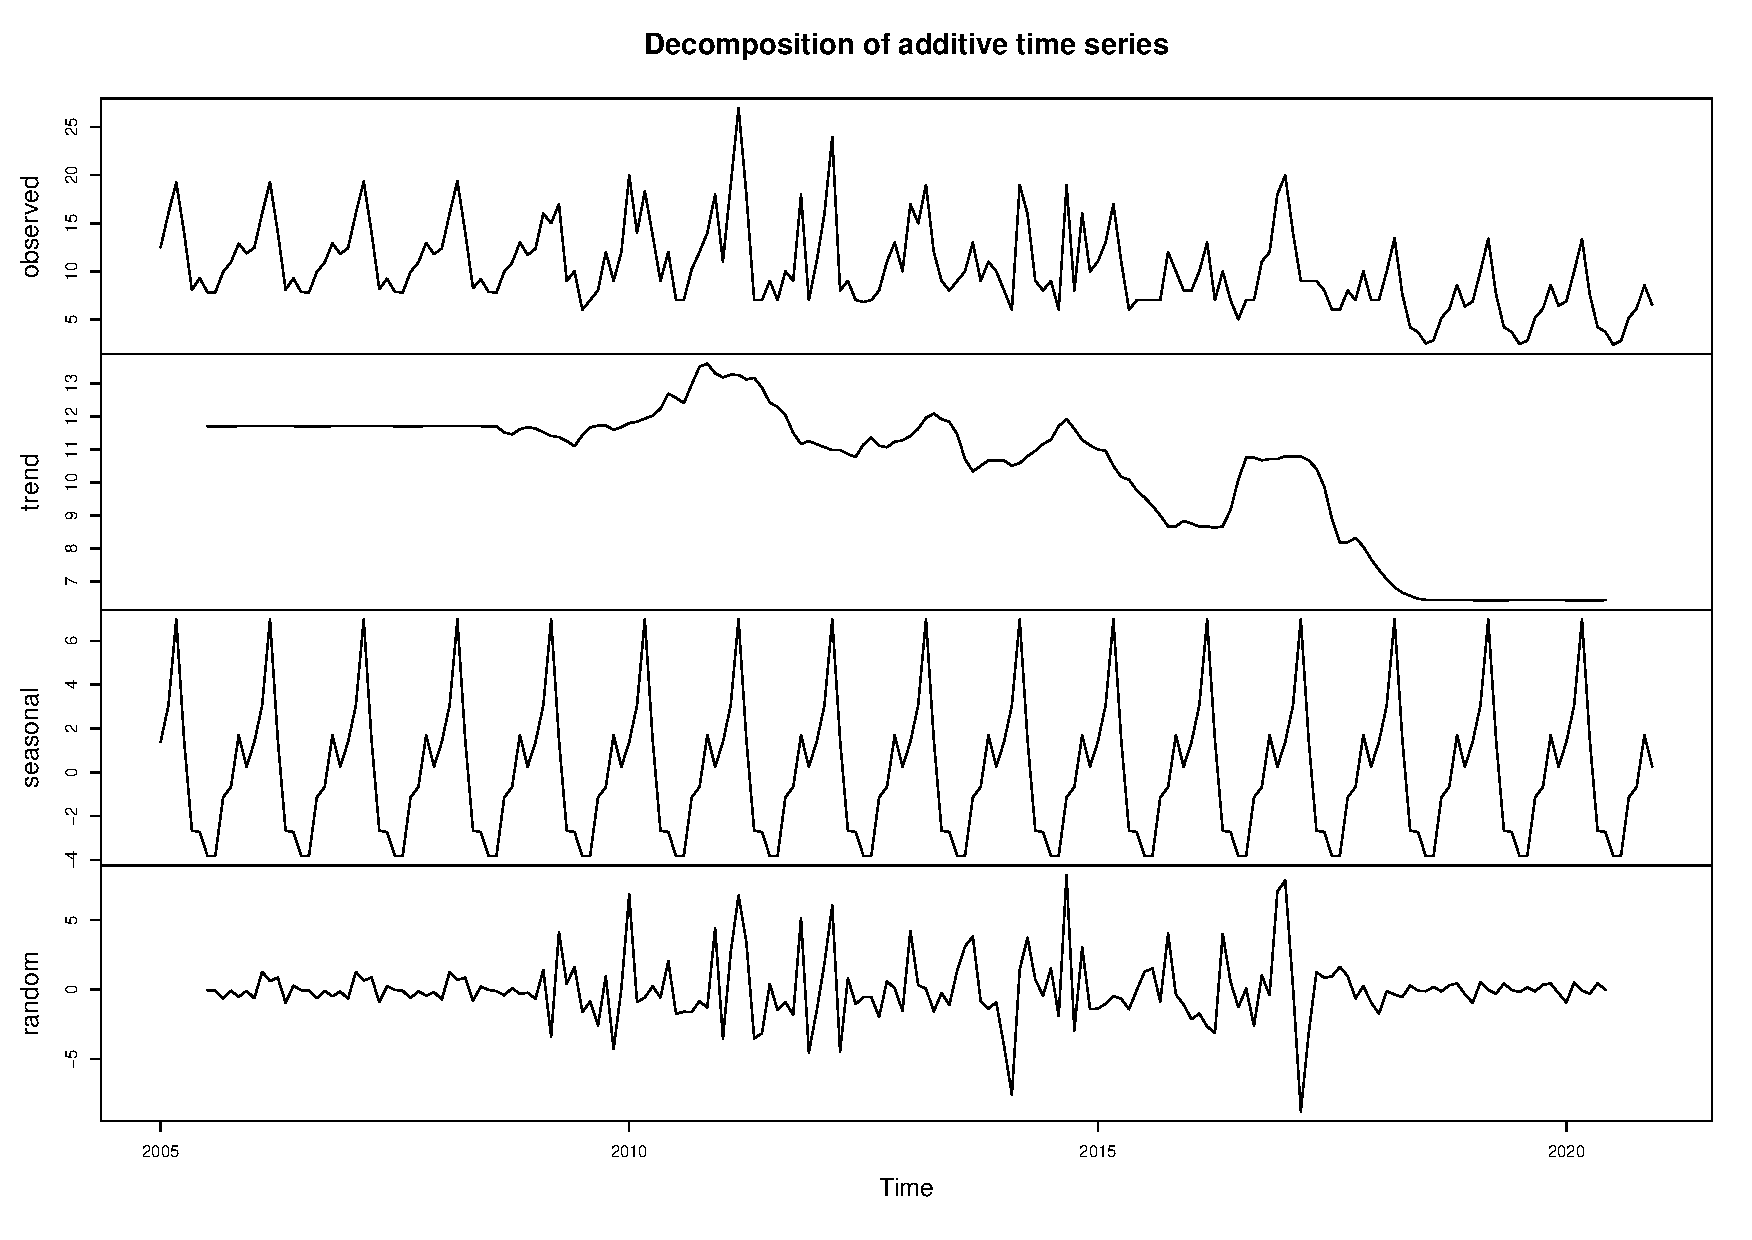
\includegraphics[width=\linewidth]{Images/London Westminster ts.pdf}
        \caption{Decomposed Additive Time Series for London Westminster}
        \label{fig:LWts}
    \end{subfigure}%
    \begin{subfigure}{.5\textwidth}
        \centering
        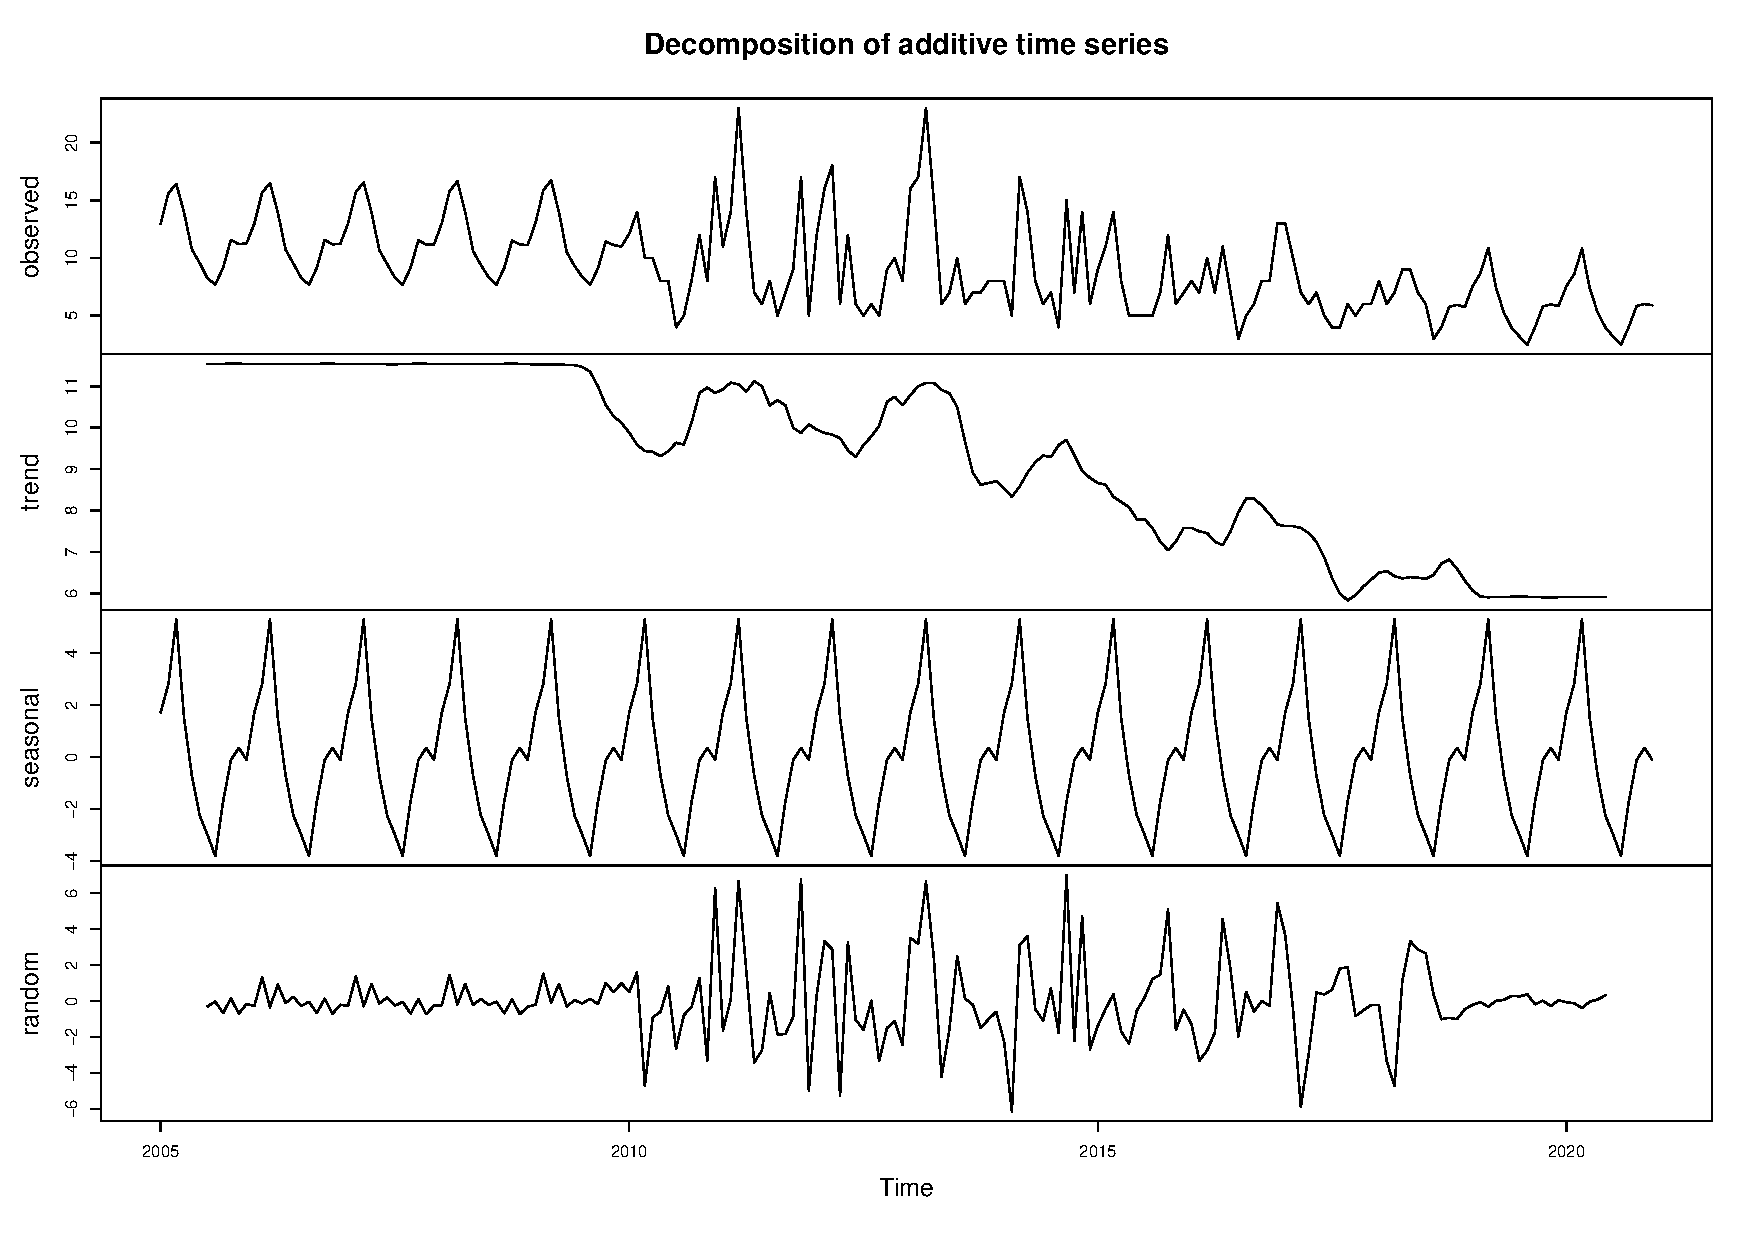
\includegraphics[width=\linewidth]{Images/Wrexham ts.pdf}
        \caption{Decomposed Additive Time Series for Wrexham}
        \label{fig:Wts}
    \end{subfigure}
\caption{Interpolated and Decomposed Time Series for 6 PM2.5 Monitoring Stations}
\label{fig:decompts}
\end{figure}

From the decomposed time series plots for each UK PM$_{2.5}$ monitoring station, there are a number of findings:
\begin{itemize}
    \item An overall decreasing trend in national PM$_{2.5}$ concentrations.
    \item A yearly seasonality, peaking around February and lowest in summer.
    \item A relatively large random error.
\end{itemize}
These findings should be taken into consideration for further work, especially when interpolating missing data points prior to 2010 and within calendar years, and also considering other factors that could be contributing to the large errors.